\documentclass[t]{beamer}
\usepackage{amsmath}
\usepackage{amsthm}
\usepackage[T1]{fontenc}
\usepackage{lmodern}
\usepackage{color}
\usepackage{xcolor}
\usepackage{hyperref}
\usepackage{multirow,varwidth} % used for SL table
\usepackage{tikz}
\usepackage{multicol}
\usepackage{graphicx}
\usepackage{etoolbox}
\usepackage{bm}
\usepackage[abs]{overpic}
\usepackage{pict2e}
\usepackage{animate}
\usepackage{verbatim}
\usepackage{soul}
\usepackage{xmpmulti}
\usepackage{subfig}
\usepackage{media9}

\makeatletter
\preto{\appendix}{%
  \patchcmd{\beamer@continueautobreak}{\refstepcounter{framenumber}}{}{}{}}
\makeatother

\usetikzlibrary{arrows,shapes}

% Making tikz overlay aware
\usetikzlibrary{positioning}
\tikzset{onslide/.code args={<#1>#2}{%
  \only<#1>{\pgfkeysalso{#2}} % \pgfkeysalso doesn't change the path
}}
\tikzset{temporal/.code args={<#1>#2#3#4}{%
  \temporal<#1>{\pgfkeysalso{#2}}{\pgfkeysalso{#3}}{\pgfkeysalso{#4}} % \pgfkeysalso doesn't change the path
}}
\tikzstyle{nuisance}=[fill=black!40!green]
\tikzstyle{onestep}=[fill=black!30!blue]
\tikzstyle{nuisance2}=[fill=white!80!green,draw=black]
\tikzstyle{nuisance2new}=[fill=black!40!green,draw=black]
\tikzstyle{onestep2}=[fill=black!30!blue,draw=black]

\newcommand\blfootnote[1]{%
  \begingroup
  \renewcommand\thefootnote{}\footnote{#1}%
  \addtocounter{footnote}{-1}%
  \endgroup
}

\newlength{\wideitemsep}
\setlength{\wideitemsep}{\itemsep}
\addtolength{\wideitemsep}{0.15em}
\let\olditem\item
\renewcommand{\item}{\setlength{\itemsep}{\wideitemsep}\olditem}

\newcommand{\norm}[1]{\left\lVert#1\right\rVert}
\newcommand{\sg}{\textnormal{sg}}


\usetheme{PaloAlto}
\usecolortheme{spruce}
\newenvironment{withoutheadline}{
\setlength{\headheight}{0pt}
\setbeamertemplate{headline}{}}

\setbeamercolor*{block title example}{fg=white,
bg= black!30!blue}
\setbeamercolor*{block body example}{fg=black,
bg= blue!5}

\setbeamertemplate{frametitle continuation}{}

 \setbeamertemplate{footline}{}

\setbeamertemplate{itemize items}[circle]
\setbeamertemplate{navigation symbols}[only frame symbol]
\setbeamerfont{framesubtitle}{size=\large}

\newtheorem{assumption}{Assumption}

%%%Set up custom notes pages %%%
\setbeamertemplate{note page}{%
  \insertnote%
}
\newcommand{\pl}{\parallel}
\newcommand{\openr}{\hbox{${\rm I\kern-.2em R}$}}
\newcommand{\nl}{\newline}
\newlength{\parskipbackup}
\setlength{\parskipbackup}{\parskip}
\newlength{\parindentbackup}
\setlength{\parindentbackup}{\parindent}
\let\notebackup\note
\renewcommand{\note}[1]{\notebackup{%
	\mode<handout>{\addtocounter{page}{-1}}%
	\setlength{\parindent}{0ex}%
	\setlength{\parskip}{10pt}%
	\noindent%
	{\normalsize{}#1}%
	\setlength{\parskip}{\parskipbackup}%
	\setlength{\parindent}{\parindentbackup}%
}%
}
\DeclareMathOperator{\sgn}{sgn}
\DeclareMathOperator{\IF}{IF}
\DeclareMathOperator{\Var}{Var}
\newcommand{\E}{\mathbb{E}}
\newcommand{\Rem}{\textnormal{Rem}}
\newcommand{\IC}{\textnormal{IC}}
\newcommand{\argmax}[1]{\underset{#1}{\operatorname{argmax}}\;}
\newcommand{\argmin}[1]{\underset{#1}{\operatorname{argmin}}\;}
%%% End Set up custom notes pages %%%

%Bibliography
\usepackage{natbib}
\bibpunct{(}{)}{,}{a}{}{;}
\usepackage{bibentry}
\nobibliography*

\title{Highly Adaptive Lasso}
%\subtitle{In Causal Inference}
\author{Mark van~der~Laan}


\institute{{\footnotesize Jiann-Ping Hsu/Karl E. Peace Professor in Biostatistics \& Statistics \\ University of California, Berkeley}}

\date{May 14, 2024, ACIC\\
%\date{December 9, 2020\\{\scriptsize FDA Webinar}
%\
\ \\
Acknowledgements: Rachael Phillips and Lars van der Laan}
%}

\usepackage{xcolor}
\hypersetup{
    colorlinks,
    linkcolor={black!50!black},
    citecolor={blue!50!black},
    urlcolor={blue!80!black}
}
\hypersetup{frenchlinks=true}


\begin{document}

\begin{frame}[noframenumbering]
\titlepage
\end{frame}

\section{$0$-HAL-MLE}

%\begin{frame\frametitle{Traditional Lasso Estimator}\begin{itemize}    \item Advantages:     \begin{itemize}        \item $L_1$-regularization performs both variable selection and penalized regression         \item Interpretable        \item Cross-validated selection of $L_1$-norm/penalty parameter   \end{itemize}  \item Disadvantages:     \begin{itemize}       \item Reliance on parametric forms places strong assumptions on the functional relationships between variables    \end{itemize}\end{itemize}\end{frame}

%\begin{frame}\frametitle{HAL Advantages}\begin{itemize}    \item First estimator that guarantees asymptotically efficient estimation of any pathwise differentiable estimand\footnote{An estimand that is a weakly differentiable functional of the density of the data, the case for most causal inference estimands under positivity.} (e.g., the average causal effect or treatment-specific survival), without enforcing strong smoothness conditions.  \item Assumptions are exceedingly mild, and expected to hold in almost every practical application.   \item Can be implemented with standard Lasso software.   \item Converges to true function at rate $n^{-1/3}(\log n)^{d/2}$.    \item Accommodates a variety of function space specifications.
    % \item Can be implemented for a large variety of function spaces, whose choice can be selected with cross-validation.\end{itemize}\end{frame}

%\section{Overview}

\begin{frame}
\frametitle{Zero-Order Spline Highly Adaptive Lasso (HAL)}

{\bf A maximum likelihood estimator over all, or subset of, cadlag functions with finite (sectional) variation norm.}

\begin{block}{\large{Key Ingredients}}
\begin{itemize}
\item Any stochastic relation/function we aim to learn from data can be approximated by linear combination (i.e., sum) of spline basis functions $X\rightarrow I(X>x_j)$ for knot point $x_j$.
\item The sectional variation norm (i.e., complexity) of the function is the $L_1$-norm in this representation.
\item Optimize empirical performance over all such linear models under fixed $L_1$-norm that is selected with cross-validation.
%\item Optimize empirical performance over all such linear models under fixed $L_1$-norm.
%\item The $L_1$-norm is optimally selected with cross-validation.
\vspace{.1in}
\end{itemize}
\end{block}

\blfootnote{van der Laan, Mark. "A generally efficient targeted minimum loss based estimator based on the highly adaptive lasso." The International Journal of Biostatistics (2017).}

\end{frame}

\begin{frame}{Formal representation of cadlag function as linear combination of zero order splines}
\begin{itemize}
\item A cadlag function $f\in D^{(0)}([0,1]^d)$ can be represented as
\[
f(x)=f(0)+\sum_{s\subset\{1,\ldots,d\}}\int_{(0_s,x_s]}df_s(u),\]
where $f_s(x_s)=f(x(j)I(j\in s): j=1,\ldots,d)$ is the section implied by setting coordinates outside $s$ equal to zero, and $x_s=(x(j): j\in s)$.
\item Moreover, we define the sectional variation norm of $f$ as the sum over $s$ of the variation norms of $f_s$:
\[
\pl f\pl_v^*=\sum_s\pl f_s\pl_v=\mid f(0)\mid +\sum_s \int_{(0_s,1_s]}\mid df_s(u)\mid .\]
\end{itemize}
\end{frame}
\begin{frame}
\begin{itemize}
\item Now, notice that this writes $f$ as an infinite linear combination of $x\rightarrow I(x_s\geq u)$ of zero order splines with knot-point $u\in (0_s,1_s]$ and coefficient $df_s(u)$, and that the sectional variation norm is the $L_1$-norm in this representation.
\end{itemize}
\end{frame}

\begin{frame}{HAL Provides Estimators of Large Variety of Nuisance Parameters Needed in Causal Inference}
\begin{itemize}
\item Causal Inference requires statistical estimation of nuisance functions.
\item In particular, it requires  estimation of conditional means; conditional  densities or cumulative distribution functions; intensities, conditional hazards. Standard loss functions can be employed for these.
\item Moreover, it is often possible to define risk functions that define  target functions of interest itself. For example, a variety of risk functions have been proposed for the conditional treatment effect. One can then apply HAL to minimize the empirical risk function.
\item In these cases,  estimation of the empirical risk function requires itself nuisance parameter estimation, where again HAL could be used.
\end{itemize}
\end{frame}

\begin{frame}{How to develop an HAL-MLE: parametrize target function in terms of unrestricted function}
\begin{itemize}
\item Suppose one is interested in a functional parameter $Q(P)$  such as a conditional density.
\item Select a loss function or risk function so that $Q(P)=\arg\min_Q R_P(Q)$, where, for example, $R_P(Q)=PL(Q)$ for some loss $L(Q)$.
\item $Q$ might be constrained in some ways. Therefore, find a parametrization $Q=Q_f$ in terms of an unconstrained function $f$. For example, parametrize a conditional density in terms of conditional hazard and represent the latter as $\exp(f)$.
\item Now, model $f$ as a linear combination of zero order splines and compute the MLE
$\beta_n=\arg\min_{\beta,\pl\beta\pl_1<C_n}R_n\left (Q_{\sum_j \beta(j)\phi_j}\right)$,
where $R_n(Q)$ is an estimate of the risk $R_{P_0}(Q)$ such as $R_n(Q)=P_n L(Q)$.
\item The HAL-MLE of $Q_0$ is then given by $Q_n=Q_{f_n}$ with $f_n=\sum_j\beta_n(j)\phi_j$.
\end{itemize}
\end{frame}

\begin{frame}{Additive models within the cadlag function space to define subspace specific HALs}
\begin{itemize}
\item Instead of selecting the richest set of basis function such as the ones implied by knot-points
$\{X_i(s): i=1,\ldots,n,s\subset\{1,\ldots,d\}\}$, one can only model a subset ${\cal S}_1$ of all the additive functions $\tilde{f}_s(x_s)=\int I(x_s\geq u) df_s(u)$  by not including all subsets $s$ in ${\cal S}_1$.
\item If ${\cal S}_1$ represents the collection of all subsets we include, then this defines additive models $f(x_s)=f(0)+\sum_{s\in {\cal S}_1}\tilde{f}_s(x_s)$. One can then define a corresponding HAL-MLE $f_{n,{\cal S}_1}$.
\item More generally, we define $D^{(0)}({\cal R}^{0,*})$ as the linear span of $\{\phi_j: j\in {\cal R}^{0,*}\}$, and by choosing the richest set ${\cal R}^0$, we have $D^{(0)}({\cal R}^0)=D^{(0)}([0,1]^d)$.
\item We use $D^{(0)}_M({\cal R}^{0,*})$ when bounding $L_1$-norm by $M$.
\end{itemize}
\end{frame}
\begin{frame}
\begin{itemize}
\item Every choice of subset of basis functions then implies an HAL-MLE.
\item One could also first use an initial ML-algorithm, such as MARS, to learn the family of subsets, ${\cal S}_1$, that appears to be needed, and then compute the resulting HAL-MLE $f_{n,{\cal S}_1}$.
\item Of course, the screening algorithm is then part of algorithm, which needs to be respected when using cross-validation to select the $L_1$-norm or select tuning parameter of the initial screening.
\end{itemize}
\end{frame}

\begin{frame}{Example: HAL of CATE}
\begin{itemize}
\item An example of a risk function $R_{P_0}(Q)$ that is non-linear in $P_0$ is the one might use in estimation of CATE $Q_0=E_0(Y\mid A=1,W)-E_0(Y\mid A=0,W)$.
\item There are two risk functions of interest defined as $R_{1,P_0}(Q)=E_0L_{1,P_0}(Q)$ and $R_{2,P_0}(Q)=E_0L_{2,P_0}(Q)$, where
\begin{eqnarray*}
L_{1,P_0}(Q)&=& (Y-E_0(Y\mid W)-(A-E_0(A\mid W))Q(W))^2\\
L_{2,P_0}(Q)&=& (D_{P_0}-Q)^2\\
D_{P_0}(O)&=& \frac{2A-1}{P_0(A\mid W)}(Y-E_0(Y\mid A,W))\\
&&+E_0(Y\mid A=1,W)-E_0(Y\mid A=0,W)
\end{eqnarray*}
\item Both loss functions are double robust w.r.t. misspecification of the nuisance parameters $P_0(A\mid W)$ and $E_0(Y\mid A,W)$.
\end{itemize}
\end{frame}
\begin{frame}
\begin{itemize}
\item Their risk based dissimilarities are $E_0(Q-Q_0)^2g_1(1\mid W)g_0(0\mid W)$ and $E_0(Q-Q_0)^2$, respectively.
\item Given the nuisance parameter estimators,  the initial rich starting model $D^{(k)}({\cal R}_N)$, the corresponding HAL-MLEs of $Q_0$  are defined as
\[
Q_{n,j}=\arg\min_{Q\in D^{(k)}_{M_n}({\cal R}_N)}P_n L_{j,n}(Q).\]
\end{itemize}
\end{frame}

\begin{frame}
\frametitle{Finite Sample Performance is Good}
\vspace{-5pt}
\begin{center}
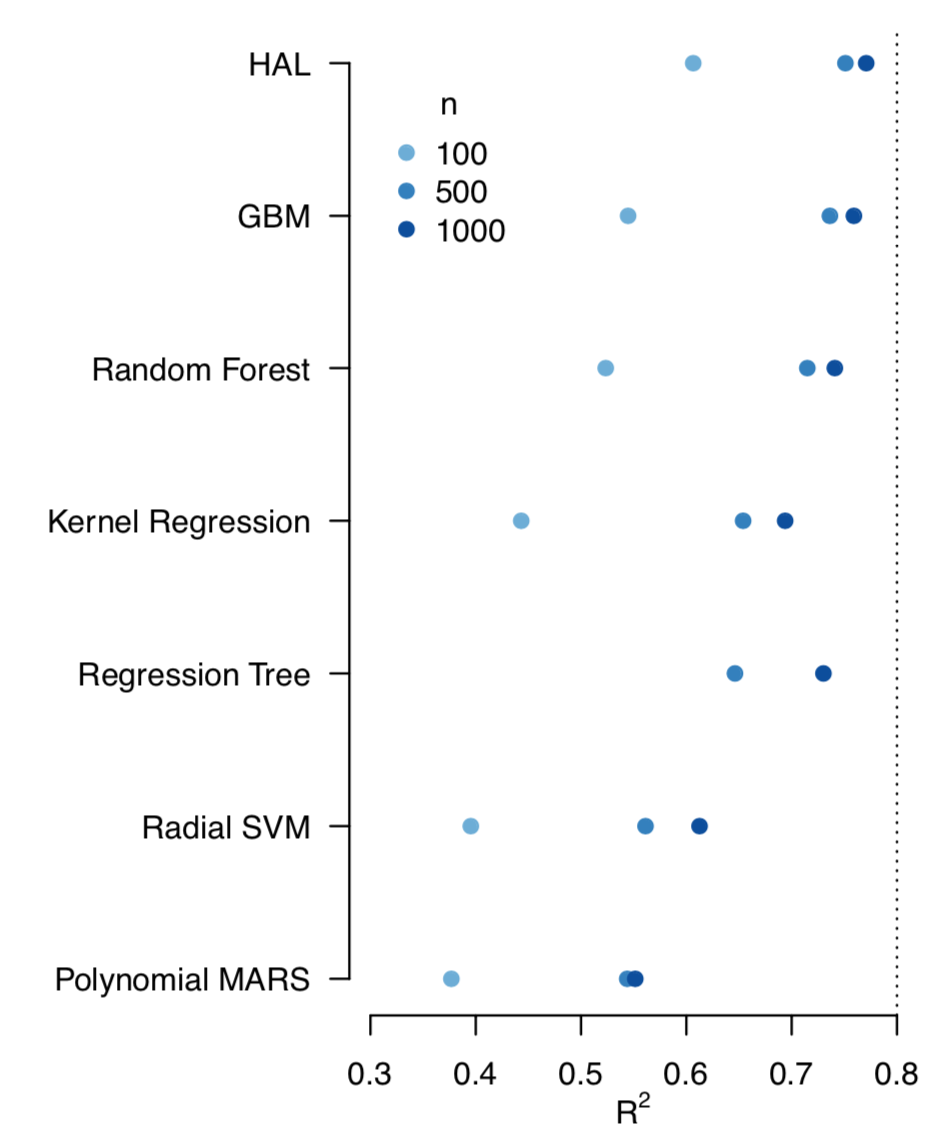
\includegraphics[width=.6\textwidth]{HAL-works.png}
\end{center}
\end{frame}

\begin{frame}
\frametitle{Illustration in Low Dimensions}
\vspace{-5pt}
\begin{center}
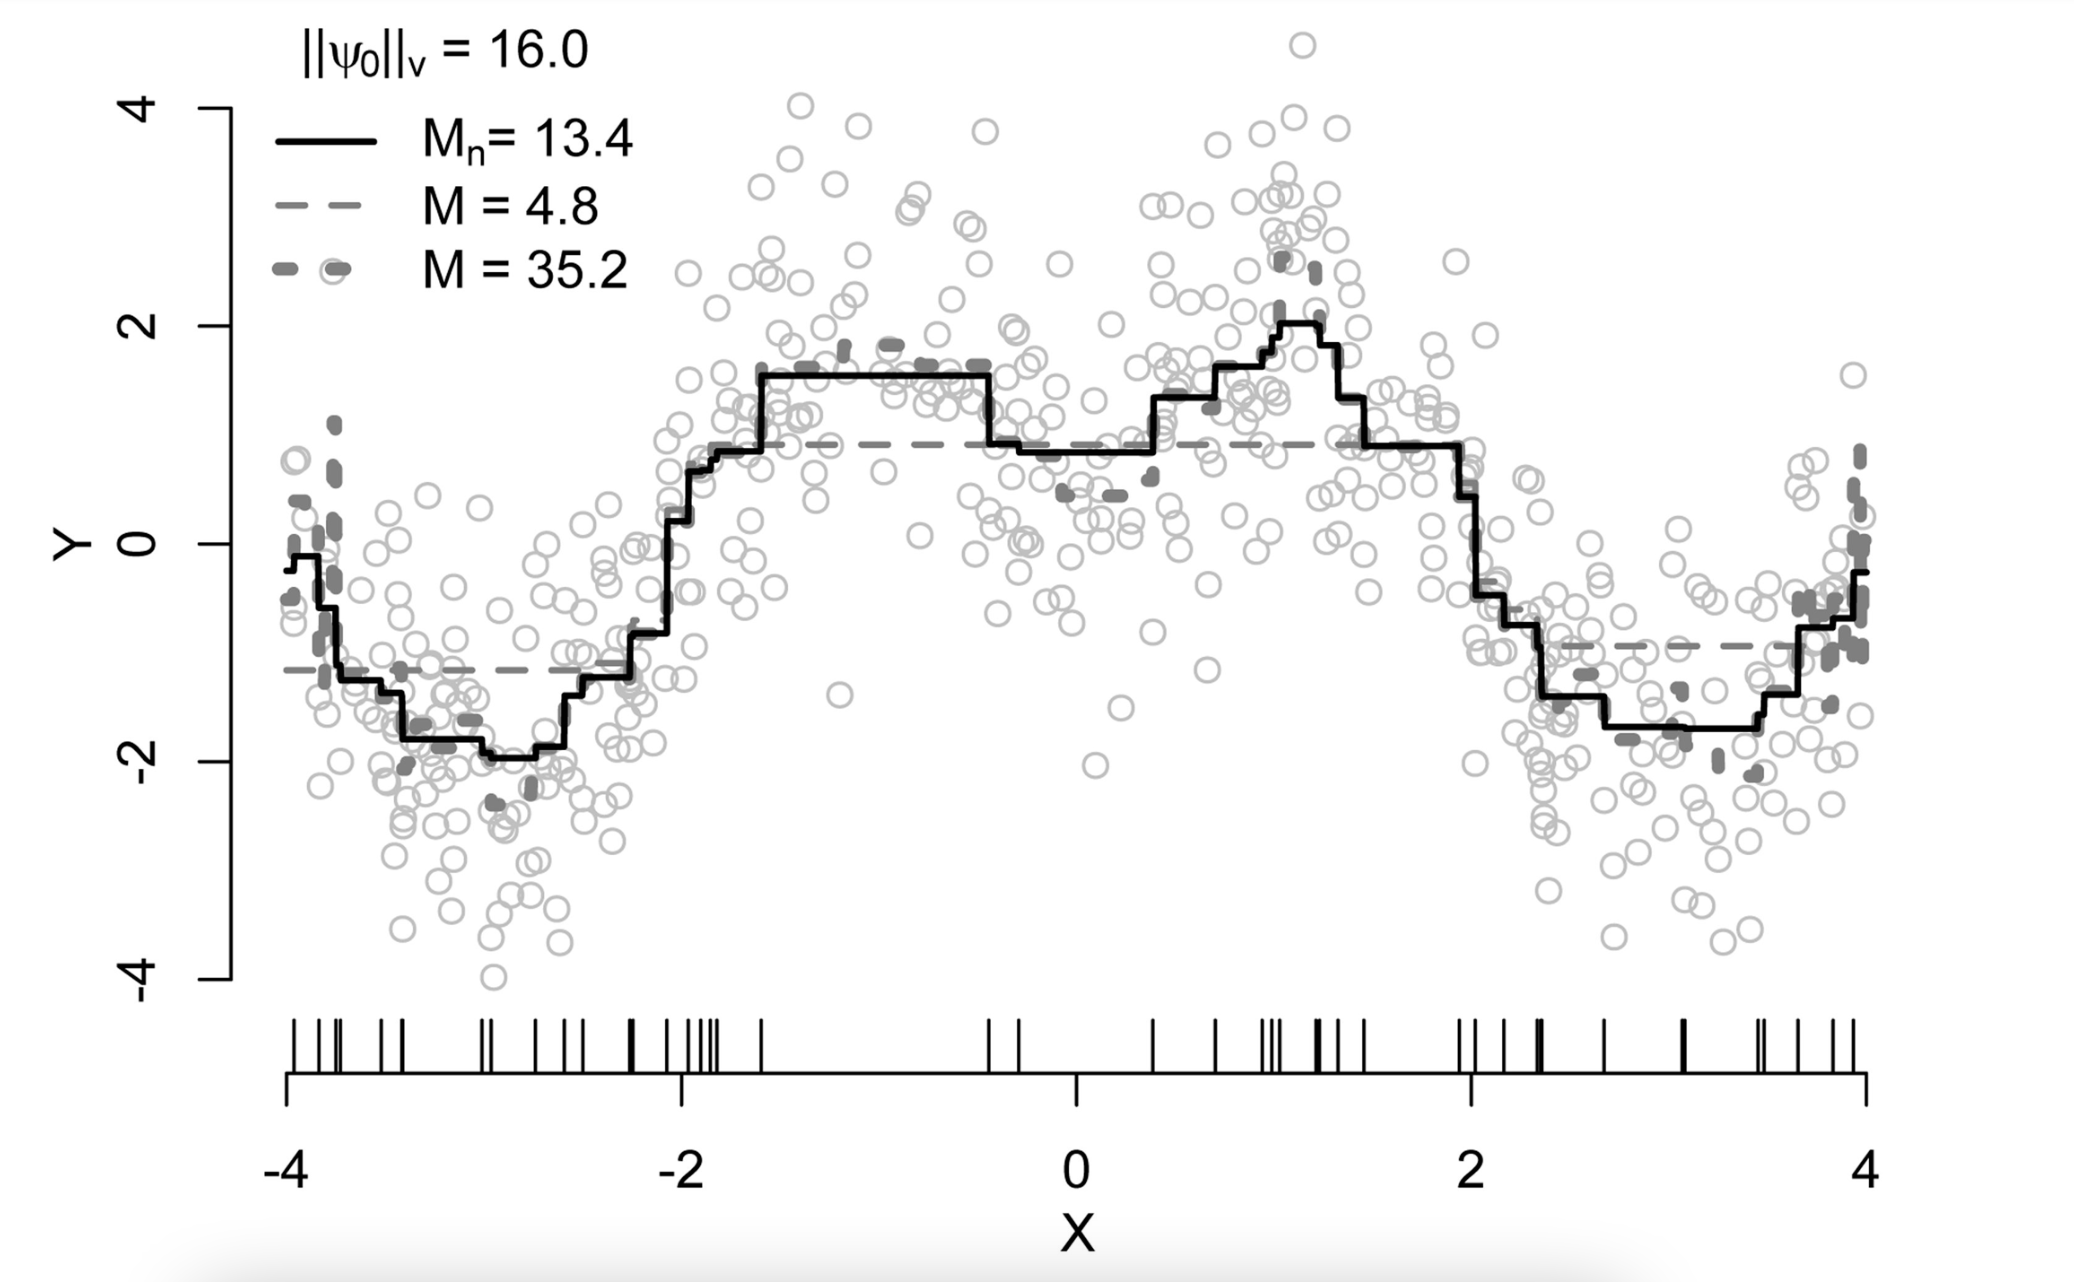
\includegraphics[width=1.1\textwidth]{HAL-univariate.png}
\end{center}
\end{frame}


\begin{frame}{Rate of convergence of zero order HAL}
\begin{itemize}
\item Let $Q_n=Q_{f_n}$ be the HAL-MLE.
\item Let $d_0(Q,Q_0)=P_0L(Q)-P_0L(Q_0)$ be the loss based dissimilarity.
\item We  have
\begin{eqnarray*}
d_0(Q_n,Q_0)&=&P_n\{ L(Q_n)-L(Q_0)\}\\
&&-(P_n-P_0)\{L(Q_n)-L(Q_0)\}\\
&\leq &- (P_n-P_0)\{L(Q_n)-L(Q_0)\}.
\end{eqnarray*}
\item Let ${\cal F}=\{L(Q_f)-L(Q_0):f\in D^{(0)}_M([0,1]^d)\}$.
\item The (known) covering number for $D^{(0)}_M([0,1]^d)$ implies the same covering number for ${\cal F}$.
\end{itemize}
\end{frame}

\begin{frame}{Using empirical process theory:}
\begin{itemize}
\item Let ${\cal F}(\delta)=\{f\in {\cal F}: P_0f^2\leq \delta^2\}$.
\item $\sup_{f\in {\cal F}(\delta)}\mid n^{1/2}(P_n-P_0)f\mid$ can be bounded by  the entropy integral
$J(\delta,{\cal F}(\delta))=\int_{(0,\delta]}\sqrt{\log N(\epsilon,{\cal F},L^2)} d\epsilon$, which behaves as $\delta^{1/2}$ up till $\log \delta$-factor.
\item Using that $P_0(L(Q)-L(Q_0)))^2\leq C d_0(Q,Q_0)$, we can then apply an iterative proof bounding \begin{eqnarray*}
d_0(Q_n,Q_0)&\leq& n^{-1/2}\sup_{f\in {\cal F}(\delta^k)}\mid n^{1/2}(P_n-P_0)f\mid\\
&\sim & n^{-1/2} J(\delta^k,{\cal F}),\end{eqnarray*}
 starting with $\delta^0=1$, $\delta^1=n^{-1/4}$, and so on.
  \end{itemize}
 \end{frame}
 \begin{frame}
 \begin{itemize}
 \item The monotone improving (in rate) sequence converges to the fixed point $\delta^*$ of equation
 \[
 \delta^2=n^{-1/2}J(\delta,{\cal F}).\]
 \item
This $\delta^*$ equals the rate of convergence for $d_0^{1/2}(Q_n,Q_0)$.
\item We find $d_0(Q_n,Q_0)=O_P(n^{-2/3}(\log n)^d)$.
\end{itemize}
\end{frame}
\section{$k$-HAL-MLE}
\begin{frame}{Derivation of first order spline representation of cadlag function}
\begin{itemize}
\item In the presentation of $f\in D^{(0)}_M([0,1]^d)$ there appear integrals
$\int_{(0(s),x(s)]} df_s(u)$.
\item Assume and write $df_s(u)=df_s/du du$; assume the RN-derivative $f_s^{(1)}=df_s/du\in D^{(0)}_M([0,1]^d)$, and plug-in the zero order spline representation for  \[
f_s^{(1)}(u)=f_s^{(1)}(0)+\sum_{s_1\subset s}\int_{(0(s_1),u(s_1)]} df_{s_1}^{(1)}(u_1).
\]
\item Apply Fubini's theorem to the double integrals over $(u,u_1)$ to obtain a representation in terms of tensor products of {\bf first} order splines.
\end{itemize}
\end{frame}
\begin{frame}
\begin{itemize}
\item As an example, let's do it for a univariate function:
\[
\begin{array}{l}
f(x)=f(0)+\int_{(0,x]} df(u)\\
= f(0)+\int_{(0,x]} f^{(1)}(u) du\\
=f(0)+\int_{(0,x]} \{f^{(1)}(0)+\int_{(0,u]} df^{(1)}(u_1)\} du\\
= f(0)+x f^{(1)}(0)+\int_{u_1}\int_u I(u\leq x) I(u_1\leq u) du df^{(1)}(u_1)\\
=f(0)+f^{(1)}(0) x+\int_{u_1} I(x\geq u_1)(x-u_1) df^{(1)}(u_1),
\end{array}
\]
which is a linear combination of first order splines $\phi^1_{u_1}(x)=I(x\geq u_1)(x-u_1)$, including $\phi^1_0(x)=x$ implied by knot-point $u_1=0$.
\end{itemize}
\end{frame}
\begin{frame}
\begin{itemize}
\item In this manner we obtain the following first order spline representation for a function
$f\in D^{(1)}([0,1]^d)$ (a cadlag function satisfying our first orders smoothness assumption):
\[
\begin{array}{l}
f(x)=f(0)+\sum_{s\subset \{1,\ldots,d\}} \phi^1_0(x(s))f^{(1)}_s(0)\\
+
\sum_{s,s_1\subset s, \mid s_1\mid>0}\bar{\phi}_{s,s_1}(x)\int \phi^1_{u(s_1)}(x(s_1)) f^{(1)}_{s,s_1}(du).\end{array}
\]
\item Here $\bar{\phi}_{s,s_1}(x(s/s_1))=\prod_{l\in s/s_1}x(l)$ and $f^{(1)}_{s,s_1}$ is the $s_1$-section of $f^{(1)}_s=df_s/du$.
\end{itemize}
\end{frame}
\begin{frame}
\begin{itemize}
\item Notice that finite linear part in this representation of $f$ is just parametric model in $x_1,\ldots,x_d$ and its interactions (e.g., for $d=2$, $x_1,x_2,x_1x_2$. The remaining infinite linear part is linear combination in tensor products of first order splines with interior knot-points in $(0(s_1),1(s_1)]$ while having knots at 0 for components $x_j$ with $j\in s/s_1$.
\item The $L_1$-norm  of all coefficients $f^{(1)}_{s,s_1}(du)$ and $f^{(1)}_s(0)$ defines our first order sectional variation norm $\pl f\pl_{v,1}^*$.
\item $D^{(1)}_M([0,1]^d)$ is defined as all functions $f\in D^{(0)}([0,1]^d)$ satisfying this first order smoothness with $\pl f\pl_{v,1}^*\leq M$.
\end{itemize}
\end{frame}
\begin{frame}{(fine enough) Finite dimensional first order spline working model}
\begin{itemize}
\item For each $s\subset\{1,\ldots,d\}$, we can select knot-points
${\cal R}^1(s)\equiv  \{(0(s/s_1),X_i(s_1)): i=1,\ldots,n,s_1\subset s\}\subset [0(s),1(s)]$. The corresponding first order splines are:
\[
\{\phi^1_{u(s)}: u(s)\in {\cal R}^1(s)\}.\]
For $s_1$ the empty set this yields  $\{0(s): s\subset\{1,\ldots,d\}\}$, giving the interactions $\phi^1_{0(s)}=\prod_{j\in s}x_j$.
\item The total set of $N$ first order splines is thus;
\[
{\cal R}^1_N\equiv \{\phi^1_{u(s)}: u(s)\in {\cal R}^1(s), s\subset \{1,\ldots,d\}\}.\]
\end{itemize}
\end{frame}
\begin{frame}
\begin{itemize}
\item The initial starting model of linear combinations of first order splines is then:
\[
D^{(1)}({\cal R}^1_N)=\left\{\sum_{j\in {\cal R}^1_N}\beta(j)\phi_j: \beta\right\}.\]
\item This working model $D^{(1)}({\cal R}^1_N)\subset D^{(1)}([0,1]^d)$ represents a close approximation of $D^{(1)}([0,1]^d)$ (providing sup-norm approximations going as fast as $n^{-1/2}$).
\end{itemize}
\end{frame}

\begin{frame}{First order spline HAL}
\begin{itemize}
\item We then define
\[
\beta_n=\arg\min_{\beta,\mid \beta\mid_1\leq C_n} P_n L(Q_{f_{N,\beta}}),\]
and first order HAL $Q_n=Q_{f_{N,\beta_n}}$.
\end{itemize}
\end{frame}
\begin{frame}{Rate of convergence for first order HAL}
\begin{itemize}
\item One can select $J$ zero order splines ${\cal R}^0(J)$ so that  $D^{(0)}({\cal R}^0(J))$ yields a $O^+(1/J)$ $L^2$-approximation of
$D^{(0)}([0,1]^d)$.
\item This explains the dimension free rate of convergence $O^+(n^{-1/3})$ for the zero-order HAL.
\item One can select $J$ first order splines, ${\cal R}^1(J)$, so that $D^{(1)}({\cal R}^1(J))$ yields a $O^+(1/J^2)$ {\bf supremum norm} approximation of $D^{(1)}([0,1]^d)$.
\item The entropy integral $J(\delta, D^{(1)}_M([0,1]^d),\pl \cdot\pl_{\infty})=O^+( \delta^{3/4})$ instead of $O^+(\delta^{1/2})$ for $D^{(0)}_M([0,1]^d)$.
\item Our rate of convergence proof  yields
\[
d_0(Q_n,Q_0)=O_P^+(n^{-4/5}).\]
\end{itemize}
\end{frame}
\begin{frame}{Higher order spline HAL}
\begin{itemize}
\item Analogue as above, we can define $D^{(k)}_M([0,1]^d)\subset D^{(k-1)}([0,1]^d)$ as class of $k$-th order smooth functions with $k$-th order sectional variation norm bounded by $M$.
\item Analogue we obtain a $k$-th order spline representation for $f\in D^{(k)}([0,1]^d)$; a finite dimensional linear working model $D^{(k)}({\cal R}^k_N)$ approximating $D^{(k)}([0,1]^d)$ and a corresponding $k$-th order spline HAL-MLE:
\[
f_n=\arg\min_{f\in D^{(k)}_{M_n}({\cal R}^k_N)}P_n L(Q_f),\]
and $Q_n=Q_{f_n}$.
\item With $J$ well chosen $k$-th order spline basis functions we can obtain an $O^+(1/J^{k+1})$ sup-norm approximation of $D^{(k)}([0,1]^d)$ .
\end{itemize}
\end{frame}
\begin{frame}
\begin{itemize}
\item As a consequence, we now have $J(\delta,D^{(k)}_M([0,1]^d),\pl\cdot\pl_{\infty})=O^+(\delta^{(2k+1)/(2k+2)})$.
\item Our rate of convergence proof now yields:
\[
d_0(Q_n^k,Q_0)=O^+_P(n^{-2k^*/(2k^*+1)}),\]
with $k^*=k+1$.
\item For example, for $k=0,1,2$, we have the dimension free rates $O_P^+(n^{-1/3})$, $O_P^+(n^{-2/5})$ and $O_P^+(n^{-3/7})$, respectively.
\end{itemize}
\end{frame}
\begin{frame}{Discrete Super Learner incorporating  higher order HAL}
\begin{itemize}
    \item By varying smoothness degree $k$ and starting sets ${\cal R}^k(j)$ of basis functions, one can define many HAL-MLEs over  $D^{(k)}_C({\cal R}^k(j))$.
    \item The discrete super learner using this library of $(k,j)$-specific HAL-MLEs will perform asymptotically exact as well as the oracle choice among all these HAL estimators,  thereby achieves the rate of convergence of HAL for the unknown smoothness $k_0$  and smallest subspace $D^{(k_0)}({\cal R}_{j_0}(d))$ containing true $Q_0$.
    \item Thus this cross-validated higher order HAL-MLE is minimax {\bf smoothness adaptive} achieving the minimax smoothness adaptive rate of convergence for univariate function estimation, up till $\log n$-factors.
%    \item Can include other machine learning algorithms and parametric models as well.
\end{itemize}
\end{frame}


 \section{Asymptotic Normality}
%\begin{frame}{Asymptotic normality of higher order HAL for Target Function, van der Laan, 2023}\begin{itemize}\item We can define higher order smoothness classes $D^{(k)}_C([0,1]^d)$ with bound $C$ on $k$-th order sectional variation norm, $k=0,1,\ldots$.\item We show $D^{(k)}([0,1]^d)$ can be represented as linear span of tensor products of $\leq k$-th order spline basis functions, where $L_1$-norm represents a sectional variation norm of higher order derivatives.\item We show that a $J$-dimensional linear span $D^{(k)}_C({\cal R}^k(J))$ of cleverly chosen set ${\cal R}^k(J)$ of $k$-th order splines uniformly  approximates $D^{(k)}_C([0,1]^d)$ at rate  $O(1/J^{k^*})$ up till $\log J$-factor, $k^*=k+1$.\end{itemize}\end{frame}
\begin{frame}{Asymptotic normality of higher order HAL}
\begin{itemize}
\item Let ${\cal R}_n$ be a set of $J_n$ $k$-th order splines  providing uniform approximation error $O^+(1/J_n^{k+1})$.
\item The non-zero coefficients in the HAL-fit  does this for us when we choose a fine enough starting model.
\item In addition, HAL will select an adaptive selection that works best for $Q_0$.
\item Let $D^{(k)}({\cal R}_n)$ be the linear working model. This set yields the $O(1/J_n^{k+1})$-uniform approximation of $Q_0$.
 \item The HAL-MLE $Q_n=\sum_{j\in {\cal R}_n}\beta_n(j)\phi_j$ operates as an MLE of the oracle approximation $Q_{0,n}=\sum_{j\in {\cal R}_n}\beta_{0,n}(j)\phi_j$ in this working model.
 \end{itemize}
 \end{frame}
 \begin{frame}
 \begin{itemize}
 \item In particular, if we do the relax-HAL (refitting the selected working model without $L_1$-penalty), then it is an exact MLE of $Q_{0,n}$.
 \item One can analyze this parametric MLE $Q_n^k$ w.r.t. $Q_{0,n}$ to establish that  $(J_n/n)^{1/2}(Q_n-Q_{0,n})(x)\Rightarrow_d N(0,\sigma^2_0(x))$, while, by our uniform approximation result $|| Q_{0,n}-Q_0 ||_{\infty}\sim O^+(1/J_n^{k+1})$.
 \end{itemize}
 \end{frame}

 \begin{frame}{\bf Technical challenge in asymptotic normality proof}
 \begin{itemize}
  \item Actually, the asymptotic normality  proof runs into an asymptotically linear approximation with influence curve still random through ${\cal R}_n$ (a linear combination of the scores of $\beta_j$, $j\in {\cal R}_n$).
    \item So, the proof would have worked if $Q_n$ is an MLE of $D^{(k)}({\cal R}_n^{\#})$ for an independent ${\cal R}_n^{\#}$.
  \item  Therefore we define this independent set as the result of the same HAL applied to independent $P_n^{\#}$ sample from $P_0$.
  We then prove that the actual HAL-MLE $Q_n$ {\bf still} acts as an approximate MLE for this fixed working model $D^{(k)}({\cal R}_n^{\#})$.
 \item In this manner our pointwise asymptotic normality proof is completed.
 \end{itemize}
 \end{frame}
 \begin{frame}{Asymptotic normality and uniform rates}
 \begin{itemize}
\item By selecting $J_n\sim n^{-1/(k+2)}$, the pointwise rate equals $n^{-k^*/(2k^*+1)}$ up till $\log n$-factors.
\item At cost of another $\log n$-factor this rate is uniform in $x$.
\item Pointwise and uniform confidence intervals follow.
\item Beyond inference for $Q_0$, these results teach us that we have dimension free {\bf uniform} rates of convergence for $\pl Q_n-Q_0\pl_{\infty}=O^+(n^{-k^*/(2k^*+1)})$.
\end{itemize}

\end{frame}

\begin{frame}{Coverage Probability of HAL-based Confidence Interval by Delta Method}
    \begin{figure}
        \centering
        \includegraphics[width=0.9\textwidth]{Overall Coverage (smoothness order = 0).pdf}
        \caption{Coverage Probability of HAL-based CI (smoothness order = 0)}
        \label{fig:my_label}
    \end{figure}
\end{frame}

\begin{frame}{Coverage Probability of HAL-based Confidence Interval by Delta Method}
    \begin{figure}
        \centering
        \includegraphics[width=0.9\textwidth]{Overall Coverage (smoothness order = 1).pdf}
        \caption{Coverage Probability of HAL-based CI (smoothness order = 1)}
        \label{fig:my_label}
    \end{figure}
\end{frame}
% Example:
% d = 3,
% n = 1000
% smoothness order = 1
\begin{frame}{Coverage Probability of HAL-based Confidence Interval by Delta Method: Example of d = 3}
    \begin{figure}
        \centering
        \includegraphics[width=0.95\textwidth]{Pointwise_coverage_prob_delta.pdf}
        \caption{Pointwise Coverage Probability of HAL-based CI (d = 3; n = 1000; smoothness order = 1)}
        \label{fig:my_label}
    \end{figure}
\end{frame}

\begin{frame}{Data Generating Functions}
    \begin{align*}
        & Y = E(Y|X) + \epsilon, \epsilon \sim N(0, 0.25);\\
        &d = 1: E(Y|X) = \sin \left(\pi X^2 \text{sign}(X)\right), \\
        & \text{where }X \sim \text{Unif}(-1,1);\\
        &d = 2: E(Y|X)=\frac{1}{1+\exp\left(-(X_1-X_1 X_2)\right)},\\
        &\text{where }X_1 \sim 4Z-2, X_2 \sim Ber(0.5), Z \sim Beta(0.85,0.85); \\
        &d = 3: E(Y|X)=\frac{1}{1+\exp\left(-(-2X_1 \text{sign}(X_1>0.5)-X_3+2X_2 X_3)\right)} \\
        & \text{where } X_1 \sim Unif(-1,1), X_2 \sim Ber(0.5), X_3 \sim Unif(-1,1)\\
    \end{align*}
\end{frame}

\section{Efficient plug-in HAL}
%\subsection{Efficient Plug-in Estimation for zero-order HAL-MLE}
\begin{frame}{Efficient HAL-TMLE (vdL, Rubin, 2006)}
\begin{itemize}
\item Construct initial estimator ${\bf P}_n$; determine a least favorable path $\{{\bf P}_{n,\epsilon}:\epsilon\in (-\delta,\delta)\}\subset {\cal M}$ through ${\bf P}_n$ with score $D^*_{{\bf P}_n}$ at $\epsilon =0$.
\item Compute MLE $\epsilon_n =\arg\max_{\epsilon}P_n L({\bf P}_{n,\epsilon})$, where $L(P)$ is a valid loss function so that $\Psi(\arg\min_P P_0L(P))=\Psi(P_0)$.
\item Let ${\bf P}_n^*={\bf P}_{n,\epsilon_n}$. The TMLE is given by $\Psi({\bf P}_n^*)$.
\item By construction, $\Psi({\bf P}_n^*)-\Psi(P_0)=(P_n-P_0)D^*_{{\bf P}_n^*}+R({\bf P}_n^*,P_0)$, with $R(P,P_0)\equiv \Psi(P)-\Psi(P_0)-(P-P_0)D^*_P$ an exact second order remainder.
\item Using the Highly Adaptive Lasso as initial estimator ${\bf P}_n$, we are guaranteed that $\Psi({\bf P}_n^*)$ is asymptotically efficient estimator of $\Psi(P_0)$ (van der Laan, 2017).
\end{itemize}
\end{frame}
\begin{frame}{HAL-TMLE of Target Estimands is Asymptotically Efficient}
\begin{itemize}
\item TMLE is two-stage method for constructing plug-in efficient estimators $\Psi(P_n^*)$ of  a pathwise differentiable target estimand $\Psi(P_0)$.
\item
The HAL-TMLE (using HAL as initial estimator) is efficient in great generality (vdL, 15).
\item  The only necessary model assumptions are:
\begin{itemize}
\item The true nuisance parameters have finite sectional variation norm
\item The loss functions of the true nuisance parameters are uniformly bounded, so that oracle inequality applies
\item The strong positivity assumption holds
\end{itemize}
\end{itemize}
\end{frame}

\begin{frame}{Example: Asymptotic  efficiency of (zero-order) HAL-TMLE for treatment-specific mean / ATE}
Consider the HAL-TMLE of $EY_1=EE(Y\mid A=1,W)$ based on $(W,A,Y)\sim P_0$ in a nonparametric statistical model.

\vspace{.15in}

It is asymptotically efficient if
\begin{enumerate}
\item $\delta<P_0(A=1\mid W)$ for some $\delta>0$
\item $W\rightarrow E_0(Y\mid A=1,W)$  and $W\rightarrow P_0(A=1\mid W)$ are cadlag
\item $W\rightarrow E_0(Y\mid A=1,W)$  and $W\rightarrow P_0(A=1\mid W)$ have finite sectional variation norm.
\end{enumerate}
\end{frame}

\begin{frame}
\frametitle{Coverage of zero-order HAL-TMLE when randomly selecting data distributions}
\vspace{-15pt}
\begin{center}
\includegraphics[width = 1\textwidth]{coverageByN.pdf}
\end{center}
\end{frame}

\begin{frame}{Undersmoothed HAL-MLE   is efficient uniformly over large class of target estimands}
\begin{itemize}
%\item Theoretical properties of O-HAL-TMLE (super-efficiency!).
\item HAL-MLE is efficient for pathwise differentiable target estimands, if $L_1$-norm is chosen large enough.
%\item Using HAL in the meta-learning step of the super learner to determine the best functional combination of candidate estimators: Meta-HAL SL.\item Meta HAL-SL is efficient for pathwise differentiable target estimands if $L_1$-norm in meta-HAL is chosen large enough.
\item Due to being an MLE, it solves a large class of score equations, in particular, efficient scores corresponding with target estimands.
\item By undersmoothing enough, it uniformly solves a class of score equations that approximates all scores with finite variation norm. As a consequence, it is a globally efficient MLE across most pathwise differentiable features.
\item This results can be applied to different assumed subspaces (i.e.., additive models of form $D^{(0)}({\cal R}(d))$) of $D^{(0)}([0,1]^d)$.
\end{itemize}
\end{frame}

\section{Bootstrapping HAL}
%\subsection{Nonparametric Bootstrap for zero-order HAL-MLE or HAL-TMLE}
\begin{frame}{Nonparametric  Bootstrap of HAL-TMLE or HAL-MLE}
\begin{itemize}
\item Fix $M$ at the cross-validation selector $M_n$ or another selector.
\item Draw 10,000 samples of size $n$ from empirical measure $P_n$.
For each bootstrap sample $P_n^{\#}$, recompute the HAL-TMLE$(M)$, say ${\bf P}_{n,M}^{\#*}$.
\item The HAL on bootstrap sample can be restricted to only include indicator basis functions that were selected by HAL-MLE$(M)$ on original data.
\item Use sampling distribution of $\psi_{n,M}^{\#*}=\Psi({\bf P}_{n,M}^{\#*})$, conditional on $P_n$, to construct $0.95$-confidence interval.
\item Increase $M$ till plateau in confidence interval for optimal coverage.
\end{itemize}
\end{frame}

%\begin{frame}{Nonparametric Bootstrap works for HAL-MLE}\begin{itemize}\item Let \[d_n(P,{\bf P}_n)=P_n L(P)-P_nL({\bf P}_n)\]be the empirical loss-based dissimilarity between a candidate $P$ and the HAL-MLE ${\bf P}_n$.\item We have $d_n({\bf P}_n^{\#},{\bf P}_n)=O_P(n^{-1/2-\alpha(d)})$:  The bootstrap HAL-MLE ${\bf P}_n^{\#}$ converges as fast to the HAL-MLE ${\bf P}_n$, but w.r.t. empirical loss-based dissimilarity.\item In addition, this empirical dissimilarity $d_n(P,{\bf P}_n)$ behaves as a square $L^2(P_n)$-norm of difference between $P$ and ${\bf P}_n$, so that it is as powerful as the dissimilarity $d_0({\bf P}_n,P_0)$ for the HAL-MLE itself.\end{itemize}\end{frame}
 \begin{frame}{Bootstrap works for HAL-TMLE or HAL-MLE}
 \begin{itemize}
 \item Conditional on the data $(P_n:n\geq 1)$, the bootstrap sampling distribution of  $\psi_n^*$ converges to optimal normal limit distribution $N(0,\sigma^2_0)$.
 \item The approximation error of bootstrap is driven by performance of nonparametric bootstrap for an empirical process indexed by Donsker class (i.e., cadlag functions with sectional variation norm bounded by $M$).
 \item This suggests  robust finite sample behavior of the nonparametric bootstrap.
 \end{itemize}
 \end{frame}\begin{frame}{Case Study}

%Two parameters:\begin{enumerate} \item Average treatment effect: Second order remainder $R(P,P_0)$ is double robust.  \item Average density value: Second order remainder $R(P,P_0)=\int (p-p_0)^2 d\mu$,
%  \item Blip variance\end{enumerate}

Compare two confidence intervals for ATE $EY_1-EY_0$:
\begin{enumerate}
\item Wald-type
\item HAL-TMLE bootstrap, using plateau selection of $L1$-norm in HAL.
\end{enumerate}

\end{frame}

\begin{frame}{Simulation}

Setting:
\begin{itemize}
  \item $W \sim N(0, 4^2, -10, 10)$ drawn i.i.d. from a truncated normal distribution, bounded within [-10,10].
  \item $A \sim Bernoulli(p(W))$ with probability p(W) as a function of W bounded between [0.3, 0.7], given by $p(W) = 0.3 + 0.1Wsin(0.1W) + \varepsilon$, $\varepsilon \sim N(0,0.05^2)$
  \item $Y = 3sin(a_1 W) + A + \varepsilon_2$ is a sinusoidal function of W, where $\varepsilon_2 \sim N(0,1)$.
  \item $a_1$ controls the frequency (and true sectional variation norm) of the sinusoidal function.
\end{itemize}
The value of the parameter of interest, the ATE, is $1$.

\begin{itemize}
    \item The experiment is repeated 500 times, and interval coverages are computed
\end{itemize}

\end{frame}

\begin{frame}{Simulation for $n=100$}
\begin{figure}
\centering
\includegraphics[scale=0.31]{HAL-bootstrap.pdf}
%\includegraphics[scale=0.4]{./fig_wilson/simu/coverage-ate-1e2.pdf}\\
%\includegraphics[scale=0.4]{./fig_wilson/simu/width-ate-1e2.pdf}
\caption{Coverage (left) and interval width (right) as a function of the $a_1$ coefficient (i.e., sectional variation norm) of the true data-generating distribution.}
\end{figure}
\end{frame}


%\subsection{Smoothness and Subspace Adaptive HALs}
\begin{frame}{Super-efficient estimation for smooth features of target function}
\begin{itemize}
\item The smoothness adaptive HAL (using cross-validation to select $k$ and additive submodel $D^{(k)}({\cal R}_{j_0})$) will asymptotically act like an HAL for an oracle smoothness $k_0$ and oracle subspace $D^{(k_0)}({\cal R}_{j_0}(d))$.
\item As a consequence, by undersmoothing within the oracle subspace it will be plug-in efficient for smooth target features w.r.t. the oracle statistical model on the data distribution that assumes $Q_0\in D^{(k_0)}({\cal R}_{j_0}(d))$.
\item That is, $\Psi(Q_n)$ is asymptotically super-efficient, and is an example of the Adaptive MLE of  (Lars van der Laan et al., 2023).
\end{itemize}
\end{frame}


\section{Adaptive TMLE}
%\section{Efficient TMLE}
\begin{frame}{Finite sample robust TMLE}
\begin{itemize}
\item The current literature on TMLE has proposed various modifications of TMLE that regularize the TMLE to be better behaved in finite samples when the support is limited (i.e., practical violation of positivity assumption).
\item For example, in censored and causal inference literature: adaptive truncation; regularize TMLE step by not fully solving EIC-equation; collaborative TMLE; outcome-adaptive TMLE; super-efficient TMLE (adjusting in PS for outcome regressions $Q_n(1,W),Q_n(0,W)$, beyond a possible baseline model).
\item These proposed regularizations have in common that they all concern targeted estimation of the orthogonal nuisance function $g(P_0)$ that is needed in targeting step, while $\Psi(P_0)=\Psi_1(Q_0)$ only depends on certain factors of likelihood.
\end{itemize}
\end{frame}
\begin{frame}
\begin{itemize}
\item Typically, these variations preserve asymptotic efficiency but adapt the targeting step towards the data to carefully trade-off bias reduction with variance gain.
\item Finite sample simulations, theoretical results such as collaborative double robustness etc, have shown that these regularizations are crucial for robust finite sample behavior for poorly supported parameters.
\item However, we never developed a truly unifying approach (and super-efficiency theory)!
\item Fortunately, Lars did: Lars van der Laan et al. (2023), Adaptive debiased machine learning.
\end{itemize}
\end{frame}


%\section{Limitations of efficiency}
\begin{frame}{Limitations of Efficient Estimators such as TMLE}
\begin{itemize}
\item Due to lack of nonparametric support, if ${\cal M}$ is close to nonparametric, then
$D^*_{P_0}(o)$ can have very large values.
\item In that case, confidence intervals for standard TMLE will be wide and no significant finding can be obtained.
\item However if we would use plug-in HAL $\Psi({\bf P}_n)$ (possibly super-efficient) we might very well still find a significant true result. Somehow, the targeting step can blow up a good initial estimator.
\item This is due to an efficient estimator to be regular along all paths through $P_0$, including paths that appear to be contradicting the data.
\end{itemize}
\end{frame}

\begin{frame}{An efficient estimator cannot adapt to structure in the true data distribution}
\begin{itemize}
\item For example, suppose $O=(W,A,Y)$ and $\Psi(P)=E_PE_P(Y\mid A=1,W)$. A plug-in HAL might end up fitting an additive model for the regression $E(Y\mid A,W)$ that contains the true regression.
\item An efficient estimator of $\Psi(P_0)$ for this additive model would be well supported and have reasonable variance.
\item But an efficient estimator for a nonparametric model protects itself against any kind of fluctuation of the data distribution, and as a consequence carries out a bias reduction that ({\bf asymptotically}) holds up uniform in $P$ in a ball around $P_0$.
\item In other words, it needs to remain asympotically unbiased under fluctuations adding a 100 way interaction.
\end{itemize}
\end{frame}
%\section{Motivating example}\begin{frame}{Motivation example: Integrating RCT with Observational Data}\begin{itemize}\item Suppose we observe data on two studies indicated by $S\in \{0,1\}$: $(S_i,W_i,A_i,Y_i)$, $i=1,\ldots,n$. \item In study $S=0$, treatment is randomized, so that the ATE can be robustly estimated.\item However, the RCT is underpowered due to small control arm or small overall sample size.\item Therefore, a TMLE of the ATE based on $S=0$ only would have large confidence intervals lacking power at reasonable alternatives. \item Can we utilize the external study $S=1$ from the real world to obtain a more efficient estimator of the ATE?  Without adding assumptions!\item We revisit this example in detail later\end{itemize}\end{frame}

\begin{frame}{Lets reset benchmarks for our estimator}
\begin{itemize}
\item {\bf Super-efficient estimator:}
Suppose that we require that our estimator of $\Psi(P_0)$ is asymptotically linear at any $P_0\in {\cal M}$, and regular along paths through $P_0$ that stay in an oracle model ${\cal M}_0\subset {\cal M}$, approximated by a data adaptive submodel ${\cal M}_n$ satisfying $P_0\in {\cal M}_0$.
\item Then, we can construct ${\cal M}_0$-super-efficient estimators that still provide asymptotically valid confidence interval and are still robust under perturbations of $P_0$ that stay in the model ${\cal M}_0$.
\item {\bf Regularized efficient estimator:} If our data adaptive model ${\cal M}_n$ approximates ${\cal M}_0={\cal M}$, let the estimator behave as an efficient estimator under model ${\cal M}_n$ that approximates the a-priori specified model ${\cal M}$ as sample size converges to infinity but in a way that carefully balances finite sample bias and variance.
\end{itemize}
\end{frame}

\begin{frame}
\frametitle{Adaptive TMLE}
\begin{itemize}
\item Data adaptively learn a model ${\cal M}_n\subset {\cal M}$. Make sure that $d(P_0,{\cal M}_n)=o_P(n^{-1/4})$ (e.g., use HAL, or cross-validation selection among a large family of submodels).
\item Define the projection parameter $\Psi_{{\cal M}_n}:{\cal M}\rightarrow\openr$ defined by $\Psi_{{\cal M}_n}(P_0)=\Psi(\Pi_{{\cal M}_n}P_0)$, where $P_{0,n}\equiv \Pi_{{\cal M}_n}(P_0)=\arg\min_{P\in {\cal M}_n}P_0L(P)$ is the log-likelihood (or loss based) projection of $P_0$ onto ${\cal M}_n$.
\item Construct a TMLE $\Psi_{{\cal M}_n}(P_n^*)$ of $\Psi_{{\cal M}_n}(P_0)$ based on canonical gradient $D^*_{{\cal M}_n,P}$ of this projection parameter.
Generally speaking, for log-likelihood loss functions
$\Psi_{{\cal M}_n}(P_n^*)=\Psi(P_n^*)$ with $P_n^*\in{\cal M}_n$.
\item Provide confidence intervals for $\Psi_{{\cal M}_n}(P_0)$ as usual based on $D_{{\cal M}_n,P_0}$.
\item Possibly cross-fit, like CV-TMLE.
\end{itemize}
\end{frame}


\begin{frame}{Why does A-TMLE work: 1) standard TMLE analysis}
\begin{itemize}
\item From TMLE analysis we will have that $\Psi_{{\cal M}_n}(P_n^*)-\Psi_{{\cal M}_n}(P_0)$ behaves as $(P_n-P_0)D^*_{{\cal M}_n,P_0}$. Therefore, under an asymptotic stability condition on ${\cal M}_n$ so that $D^*_{{\cal M}_n,P_0}\rightarrow_p D^*_{{\cal M}_0,P_0}$ we have that it behaves as $P_n D^*_{{\cal M}_0,P_0}$ and is thus asymptotically normal with mean zero and variance $\sigma^2_{{\cal M}_0}(P_0)=P_0\{D^*_{{\cal M}_0,P_0}\}^2$.
\item Cross-fitting weakens this need for asymptotic stability. Moreover, one might still have asymptotic normality by standardizing by a variance estimator.
\item $D^*_{{\cal M}_0,P_0}$ equals the efficient influence curve of $\Psi:{\cal M}_0\rightarrow \openr$: i.e. we achieve the efficiency we would achieve with TMLE if we would  a priori know that $P_0\in {\cal M}_0$.
\end{itemize}
\end{frame}
\begin{frame}{Why does A-TMLE work: 2) data adaptive model bias negligible}
\begin{itemize}
\item Let $R_{{\cal M}_0}(P,P_0)=\Psi_{{\cal M}_0}(P)-\Psi_{{\cal M}_0}(P_0)+P_0 D^*_{{\cal M}_0,P}$.
\item We have
\[
\begin{array}{l}
\Psi_{{\cal M}_n}(P_0)-\Psi(P_0)=\\
(P_{0,n}-P_0)\{D^*_{{\cal M}_0,P_{0,n}}-\Pi_n(D^*_{{\cal M}_0,P_{0,n}}\mid T_{{\cal  M}_n}(P_{0,n}))\}\\
\hfill +R_{{\cal M}_0}(P_{0,n},P_0),
\end{array}
\]
where the projection $\Pi_n$ projects $D^*_{{\cal M}_0,P_{0,n}}$ onto tangent space of ${\cal M}_n$ at $P_{0,n}$.
\end{itemize}
\end{frame}
\begin{frame}
\begin{itemize}
\item This is a very nice second order remainder (i.e., $o_P(n^{-1/2})$).
\item Therefore, our adaptive TMLE is asymptotically linear estimator of $\Psi(P_0)$ with (super-efficient) influence curve $D^*_{{\cal M}_0,P_0}$.
\item Since it operates as an efficient estimator of $\Psi_{{\cal M}_n}(P_0)$ it will also be regular along any path through $P_0$ that stays in the limit oracle model ${\cal M}_0$.
\end{itemize}
\end{frame}



\section{O-A-HAL-C-TMLE}

\begin{frame}{Outcome-regression weighted LASSO (OAL)}
Shortreed \& Ertefaie (2017) proposed outcome-regression weighted Lasso (OAL) for propensity score (PS) estimation:
\begin{itemize}
\item  Fit unpenalized linear model for $\E(Y|A,W)$:
  $$(\hat{\alpha}, \hat{\eta}) = \arg\min_{\alpha,\eta} l_n(\alpha;Y,A,W).$$
where $\eta$ is the coefficient for $A$, and $\alpha$ is the coefficient for $W$.

\item Denote the coefficient for variable $W_j$ in the outcome regression with $\hat{\alpha}_j$.

  \item Fit PS with Lasso using regularization term
    \[\lambda \sum_j ||\alpha_j||^{-\gamma} ||\beta_j || \mbox{ instead of usual $\lambda \sum_j \mid \beta_j\mid$.}\]

%\item  They suggest $\gamma= 2 \cdot (3 - \lambda)$ to ensure the necessary conditions for the convergence properties.

\end{itemize}
\end{frame}


\begin{frame}
\frametitle{HAL-based OAL for PS Estimation}

The theoretical property of OAL relies on the \textbf{\textit{correct parametric formula}}, which is often unknown in practice.

\vspace{.1in}

We extend OAL to outcome-regression weighted HAL (OHAL):
%and then select weighted L1-norm with C-TMLE:
\begin{enumerate}
\item Compute the outcome regression using Lasso of form $\sum_j \alpha_n(j)\phi_j(W,A)$.
%with dependent variable the outcome $Y$ and features the basis functions $\phi_j(A,W)$ and the treatment indicator $A$.
\item Use as basis functions for the PS $\{\phi_j(1,W),\phi_j(0,W): j\}$.
\item Both of these two basis functions will be associated with same weight $\alpha_n(j)$.
%The $L_1$ constraint parameter $M^{(1)}$ can be selected by CV.
\item Compute the propensity score using a Lasso logistic regression using the above basis functions.  The $L_1$-constraint for $\beta_{j}$'s, the coefficient for $\phi_j$, is defined as the weighted $L_1$-norm above.
\item Or simply define $\pl \beta\pl_1=\sum_{j, \alpha_n(j)\not =0}\mid \beta(j)\mid$.
%  $$\sum_{s \subset \{1, %\cdots,n\}}\sum_{i=1}^{n}|\alpha_{s,i}|^{-\gamma} |\beta_{s,i}| < %M^{(2)}$$
\end{enumerate}
\end{frame}
\begin{frame}{C-TMLE to select $L_1$-norm}
\begin{itemize}
  \item Tune the $L_1$-norm with C-TMLE: i.e. optimize in $\lambda$ increase in likelihood of TMLE-step using $g_{n,\lambda}$.
\end{itemize}
\end{frame}


%\begin{frame}{Tuning of $L_1$-norm of $g_{n,\lambda}$ with Collaborative TMLE}
%The last remaining question is how can we select the tuning parameter ($M^{(1)}, M^{(2)})$, the $L_1$ constraint parameters in LASSO for the outcome model and exposure model. Here we propose using C-TMLE to tune the regularization parameter:\textbf{OHAL-CTMLE algorithm:}\begin{enumerate}\item Get the estimated coefficients $\alpha_{cv, n}$ for basis functions in the outcome regression HAL-fit.\item Select $M^{(2)}_{cv}$ with CV in the propensity score estimation based on the outcome regression coefficients $\alpha_{cv, n}$.\item Define an increasing sequence of $M^{(2)}_j, j = 1,\cdots, k$, with $M^{(2)}_1 = M^{(2)}_{cv}$ . Construct a sequence of PS estimators $G_{n,j}, j = 1,\cdots, k$ corresponding to each $M^{(2)}_j$.\item Provide the propensity score estimator sequence $G_{n,j}$ to C-TMLE in step \ref{1} to determine the optimal $M^{(2)}$.\end{enumerate}\end{frame}


\begin{frame}{OHAL Performance based on Kang \& Shafer (2007) Simulation}

\begin{itemize}
\item Pre-treatment covariates $(Z_{i1}, \cdots, Z_{i4})$ are generated from uncorrelated standard normal distributions.
\item Treatment indicator is then generated from a Bernoulli distribution with:
\begin{equation*}
  P(A_i=1 |Z_i) = \text{expit}(- Z_{i1} + 0.5 Z_{i2} - 0.25 Z_{i3} - 0.1 Z_{i4})
\end{equation*}
\item Potential outcomes are generated by:
\begin{equation*}
  \begin{aligned}
    Y_i^{(a)} &= 210 + 27.4 Z_{i1} + 13.7 Z_{i2} + 13.7 Z_{i3} + 13.7 Z_{i4} + \epsilon\\
    \epsilon & \sim N(0, 1)
  \end{aligned}
\end{equation*}
\item Thus, the value of the estimand, the ATE, is $0$.
\end{itemize}
% Continuous potential outcomes are generated as the linear combination of the pre-treatment covariates, and do not rely on the treatment $A$.

\end{frame}


\begin{frame}{Simulation to Assess OHAL Performance (Continued)}
\begin{itemize}
\item Only transformed covariates $W$ are observed:

 \begin{equation*}
       \begin{aligned}
         W_{i1}& = \exp(Z_{i1}/2) \\
         W_{i2}& = z_{i2}/(1+\exp(Z_{i1}) + 10\\
         W_{i3}& = (Z_{i1}Z_{i3}/25 + 0.6)^3\\
         W_{i4}& = (Z_2  + Z_4 + 20)^2.
      \end{aligned}
 \end{equation*}
 \vspace{.2in}
\item In our experiment, we also included an instrumental variable $W_{i5}$, and the PS was modified to:
\end{itemize}
 \begin{equation*}
  PS = \text{expit}\left(\frac{- Z_{1} + 0.5 Z_{2} - 0.25 Z_{3} - 0.1 Z_{4}}{2} + W_{5}\right)
 \end{equation*}

\end{frame}


\begin{frame}{OHAL Simulation Results}

We use main-term linear regression to create biased initial estimator $\bar{Q}_n^0$ for TMLE/C-TMLE.

\begin{table}[ht]
\centering
\begin{tabular}{l|rrrr}
  &  {\small TMLE-HAL} & {\small CTMLE-HAL} & {\small CTMLE-OHAL} & Oracle \\
   \hline \hline
N=500  & 7.06 & 6.34 & \textbf{2.94} & 3.64 \\
N=1000  & 4.42 & 3.55 & \textbf{1.40} & 1.70 \\
N=2000  & 2.94 & 1.85 & \textbf{0.83} & 0.87 \\
   \hline
\end{tabular}
\caption{MSE for each estimator across 200 replications with different sample size. }
\end{table}
% We can see CTMLE-HAL improves TMLE-HAL. CTMLE-OHAL further improves CTMLE-HAL with outcome adaptive regularization. It even achieves better performance than the oracle estimator, which is defined as TMLE with true PS.


\end{frame}



%\begin{frame}{Simulation}Results (n = 500):\begin{figure}\centering\includegraphics[scale=0.4]{./fig_wilson/simu/coverage-ate-5e2.pdf}\\\includegraphics[scale=0.4]{./fig_wilson/simu/width-ate-5e2.pdf}\caption{Coverage (upper) and interval width (lower) as a function of the $a_1$ coefficient (sectional variation norm) of the true distribution}\end{figure}\begin{itemize}  \item same take-home message as n = 100.\end{itemize}\end{frame}
\section{Efficient IPCW}

\begin{frame}{Inverse Probability of Treatment/Censoring Weighted Estimators using HAL (Ertefaije, Hejazi, vdL, 2023)}
\begin{itemize}
\item Let $O=\Phi(C,X)$, $P_X\in {\cal M}^F$, $G_{C\mid X}$ satisfying CAR, and let $\Psi^F(P_X) $ be the target.
\item One can then construct IPCW-estimators $\psi_{n,IPCW}$ as solutions of $P_n U_{G_n}(D^F(\psi))=0$ in $\psi$ with $U_G(D^F)(O)$ an inverse probability weighted full-data estimating function $D^F$ satisfying $E_G(U_G(D^F)(O)\mid X)=D^F(X)$.
\item By using undersmoothed HAL as estimator of the censoring mechanism $G$, the HAL-IPCW estimator $\psi_{n,IPCW}$  is asymptotically linear with influence curve the IPCW-function $U_G(D^F(\psi))$ minus its projection on the tangent space $T_{CAR}$.
\end{itemize}
\end{frame}
\begin{frame}
\begin{itemize}
\item In particular, for nonparametric full-data models, the IPCW-estimator using undersmoothed HAL is asymptotically efficient.
\item Similarly, if one uses HAL to estimate $G$ for double robust estimators, then inference and efficiency is preserved under misspecified estimators of the full data distribution $P_X$.
\end{itemize}
\end{frame}
\section{Meta-HAL}
\begin{frame}{Meta-HAL Super Learning (Wang, Zhang, vdL, 2024)}
\begin{itemize}
\item Given a library of candidate machine learning algorithms, one can construct a cross-fitted data set in which the covariates are the cross-fitted predictions.
\item One can then use HAL at this Meta-level.
\item This is the same as using HAL to do super-learning instead of convex linear regression.
\item One can include this Meta-HAL SL as candidates in a discrete super-learner to tune the meta-level HAL optimally.
\item Meta-HAL satisfies the same properties at HAL, but at the Meta-level: rates of convergence; plug-in efficiency; asymptotic normality.
\item This provides a powerful approach for targeting learning incorporating multimodal data sources, utilizing algorithms tailored for these data sources such as deep-learning for images etc.
\end{itemize}
\end{frame}

\section{Conclusion}
\begin{frame}{Concluding Remarks}
\begin{itemize}
    \item HAL is the first general nonparametric MLE, with formal theoretical properties analogue to parametric MLE.
      \item It represents a large class of HAL estimators by restricting function space, a priori, or data adaptively (screening).
    \item Its sparse representation makes it an excellent algorithm for interpretable machine learning.
    \item Fast dimension free rate of convergence, even uniform convergence, and has pointwise normal limit distribution.
    \item Can be made adaptive to unknown smoothness and support.
    \item HAL-TMLE is guaranteed asymptotically efficient for smooth features.
    \end{itemize}
    \end{frame}
    \begin{frame}
    \begin{itemize}
    \item Smoothness and subspace adaptive HAL super-efficient for smooth features, under conditions of the A-MLE/A-TMLE of Lars vdL et al. (2023).
     \item It yields delta-method based Wald type confidence intervals, and it allows for nonparametric bootstrap to improve finite sample coverage.
    \item It has many applications to further enhance TMLE beyond using HAL in discrete SL: e.g., outcome adaptive HAL-TMLE, higher order TMLE, Collaborative TMLE, etc.
\end{itemize}
\end{frame}


%\begin{frame}\frametitle{Frequently Asked Questions}\begin{itemize}   \item Why are global smoothing assumptions better than local smoothing assumptions?   \item If I include HAL in my Super Learner library, then why would I include anything else?    \item How does screening HAL's basis functions affect it's rate of convergence to the true function?   \item How does HAL compare to BART?\end{itemize}\end{frame}

\end{document}% Simulation Results of HAL-based CI for conditional mean functions
% Overall coverage
\begin{frame}{Coverage Probability of HAL-based Confidence Interval by Delta Method}
    \begin{figure}
        \centering
        \includegraphics[width=0.9\textwidth]{Overall Coverage (smoothness order = 0).pdf}
        \caption{Coverage Probability of HAL-based CI (smoothness order = 0)}
        \label{fig:my_label}
    \end{figure}
\end{frame}

\begin{frame}{Coverage Probability of HAL-based Confidence Interval by Delta Method}
    \begin{figure}
        \centering
        \includegraphics[width=0.9\textwidth]{Overall Coverage (smoothness order = 1).pdf}
        \caption{Coverage Probability of HAL-based CI (smoothness order = 1)}
        \label{fig:my_label}
    \end{figure}
\end{frame}
% Example:
% d = 3,
% n = 1000
% smoothness order = 1
\begin{frame}{Coverage Probability of HAL-based Confidence Interval by Delta Method: Example of d = 3}
    \begin{figure}
        \centering
        \includegraphics[width=0.95\textwidth]{Pointwise_coverage_prob_delta.pdf}
        \caption{Pointwise Coverage Probability of HAL-based CI (d = 3; n = 1000; smoothness order = 1)}
        \label{fig:my_label}
    \end{figure}
\end{frame}

\begin{frame}{Data Generating Functions}
    \begin{align*}
        & Y = E(Y|X) + \epsilon, \epsilon \sim N(0, 0.25);\\
        &d = 1: E(Y|X) = \sin \left(\pi X^2 \text{sign}(X)\right), \\
        & \text{where }X \sim \text{Unif}(-1,1);\\
        &d = 2: E(Y|X)=\frac{1}{1+\exp\left(-(X_1-X_1 X_2)\right)},\\
        &\text{where }X_1 \sim 4Z-2, X_2 \sim Ber(0.5), Z \sim Beta(0.85,0.85); \\
        &d = 3: E(Y|X)=\frac{1}{1+\exp\left(-(-2X_1 \text{sign}(X_1>0.5)-X_3+2X_2 X_3)\right)} \\
        & \text{where } X_1 \sim Unif(-1,1), X_2 \sim Ber(0.5), X_3 \sim Unif(-1,1)\\
    \end{align*}
\end{frame}

\section{Implementation}\begin{frame}\frametitle{Tuning HAL}HAL's computational cost is controlled by the number of basis functions, which can be as large as $n*2^{d-1}$.\vspace{.1in}Options for constraining the functional form of the target function:
\begin{itemize}
    \item Enforce a minimum $(p,1-p)$ with $p$ proportion of 1's in basis function.
    \item Enforce a maximal order of interaction.
    \item Specify particular additive model.
    %structure: e.g., $f(X_1,X_2,X_3)=f_1(X_1)+f_2(X_2,X_3)$.
    \item Enforce monotonicity for some of the functions.
    \item Enforce higher order splines and thereby smoothness.
    \item Discretize continuous covariates: fewer knot-points.
    \item Greedy screening: iteratively, selected $j$-th order basis functions  generate $j+1$-th order basis functions.

\end{itemize}
\end{frame}

\begin{frame}
\frametitle{Basic \texttt{R} \texttt{hal9001} Functionality}

\begin{enumerate}
    \item Load package and data: \newline \texttt{library(hal9001)} \newline
    \texttt{data(mtcars)}
    \item Create numeric vector for dependent variable: \newline \texttt{Y <-  mtcars[,"mpg"]}
    \item Create dataframe or matrix of predictors: \newline
    \texttt{X <- mtcars[,c("cyl", "disp", "hp", "wt")]}
    \item Fit HAL: \newline
   \texttt{ hal\_fit <- fit\_hal(X=X, Y=Y)}\newline
   \newline
   \small{\textit{Note}: default \texttt{max\_degree=3} considers no more than 3-way interactions, and default \texttt{reduce\_basis=0} places no restrictions on the minimum proportion of 1's in basis functions.}
\end{enumerate}
\end{frame}


\begin{frame}
\frametitle{Summary table of \texttt{hal9001}  HAL fit}
\vspace{-2pt}
\texttt{summary(hal\_fit)\$table}
\begin{center}
\vspace{-2pt}
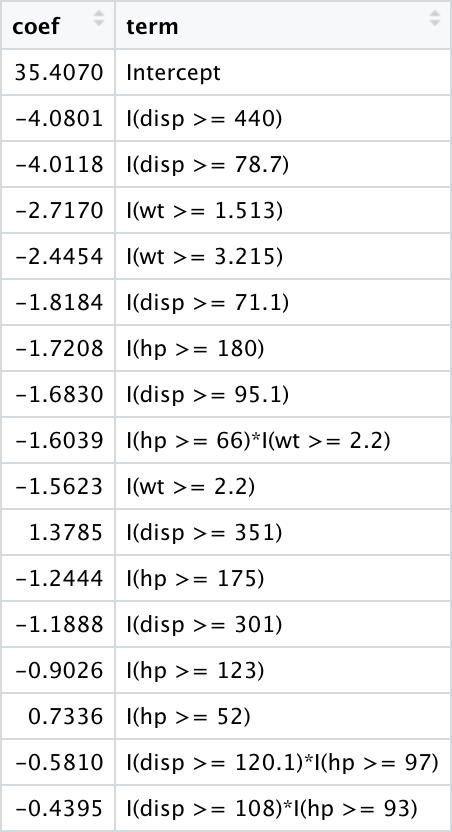
\includegraphics[width = 0.38\textwidth]{HAL-summary-mtcars.png}
\end{center}
\end{frame}

\begin{frame}
\frametitle{Specifying \texttt{hal9001} model formulas}

\textit{Example}: Observe $O=(W_1, W_2, A, Y) \sim P_0$ \newline
$$\text{\texttt{R} code: \texttt{fit\_hal(Y, X, formula, data, ...)}} $$

\textbf{Additive model \texttt{formula}}: \newline
$\text{\texttt{Y}} \sim . $ or $\text{\texttt{Y}} \sim \text{\texttt{h(W1) + h(W2) + h(A)}} $

\vspace{.05in}

\textbf{Bi-additive model \texttt{formula}}: \newline
$\text{\texttt{Y}} \sim . $\^{}$\text{\texttt{2}}$ or $\text{\texttt{Y}} \sim \text{\texttt{h(W1)+h(W2)+h(A)+h(W1,W2)+h(W1,A)+h(W2,A)}}$

\vspace{.05in}

\textbf{Only interactions with A \texttt{formula}:} \newline
$\text{\texttt{Y}} \sim \text{\texttt{h}}(.) + \text{\texttt{h}}(.\text{\texttt{,A}})$ or $\text{\texttt{Y}} \sim \text{\texttt{h(W1)+h(W2)+h(A)+h(W1,A)+h(W2,A)}}$

\vspace{.05in}

\textbf{Monotone $\uparrow$ (i) $\downarrow$ (d) \texttt{formula} examples}:

$\text{\texttt{Y}} \sim \text{\texttt{i}}(.) $ or $\text{\texttt{Y}} \sim \text{\texttt{i}}(.) + \text{\texttt{i}}(.,.) $ or
$\text{\texttt{Y}} \sim \text{\texttt{i(W1)+d(W2)+i(A)}}$
%\newline
%\newline
\end{frame}


\begin{frame}
\frametitle{Possible HAL fits under various smoothness orders}

\textit{Example}: Observe $(W, A, Y) \sim P_0$
$$\text{\texttt{R} code: \texttt{fit\_hal(Y, X, data, formula, k, ...)}} $$

\textbf{Example fits for 0-order smoothness, \texttt{k=0}}: \newline
    Additive model:

    $Y = \mathbb{I}(W>0.5) + \mathbb{I}(W > 0.3) + \mathbb{I}(A>0)$ \newline
    Bi-additive model:

    $Y = \mathbb{I}(W>0.5) + \mathbb{I}(A>0)  + \mathbb{I}(W>0.5, A>0)$
    \newline
    \newline
\textbf{Example fits for 1st-order smoothness, \texttt{k=1}}: \newline
Additive model:

$Y = \mathbb{I}(W>0.5)[W - 0.5] + \mathbb{I}(W>0.3)[W - 0.3] + \mathbb{I}(A>0)[A-0]$
  \newline
 Bi-additive model:

 $Y = \mathbb{I}(W>0.5)[W - 0.5] + \mathbb{I}(A>0)[A-0]  + \mathbb{I}(W>0.5, A>0)[W - 0.5][A - 0]$ \newline

\end{frame}


\begin{frame}
\frametitle{Performance under Various Screening Options}
\begin{itemize}
    \item Binning: Reducing number of spline knot points, separately for 1-way, 2-way, 3-way basis functions.
    \item Greedy screening: Build interactions sequentially from screened basis functions of lower order interactions.
\end{itemize}

$$n = 2000;\, d = 12$$
Size of regression matrix ($n\times p$) up to 3-way interactions: \newline
Binning (100, 25, 5): $p = 30,000$ \newline
No Binning:  $p=600,000$

\vspace{.15in}

Sequential (up to 2-way): {\small first $p$=20,000 then $p$=2,000, \newline $R^2$=0.88, MSE=0.376} \newline
No Sequential (up to 2-way): {\small $p$=150,000, $R^2$=0.85, MSE=0.394} \newline

\centering
\textit{More basis functions does not imply better performance.}
\end{frame}
